
\section{Vývojový deník robota pro Ketchup House aneb stručná historie výroby } \label{denik} \index{vývojový deník}

\textbf{Vývojový deník} je v podstatě kronika stavby robota. Silně doporučuji jej alespoň heslovitě psát s konkrétními daty. 
Při porovnání s \textbf{plánem stavby} (tj. s vizí, jak rychle se co udělá, což taky doporučuji sepsat)  je velmi cenným zdrojem zkušeností. \index{plán stavby}
Pro představu, velmi hrubý plán stavby tohoto robota byl následující: září - listopad: plán a stavba mechanická konstrukce, prosinec -- leden: zapojení elektroniky a senzorů,
únor -- duben: programování a~testování, květen -- červen: rezerva. Závěr: to se v pohodě stihne. 

O tom, jaká byla realita, čtěte dále. 

\begin{description}
	\item[září - říjen:] 
	
	\begin{itemize}
	    \item[]
		\item první návrh strategie
		\item první návrh mechaniky a konstrukce
		\item  vize ohledně senzorů
		\item jako řídící jednotka byla zvolena deska Arduino Mega, především kvůli velkému počtu pinů, cíl: vystačit si s jednou deskou  
		
	\end{itemize} 
	
	\item[listopad:] 
	
	\begin{itemize}
		\item[]
		\item druhý návrh strategie
		\item výroba první konstrukce, jsou použity vrtačkové motory
		\item pokusy o zprovoznění/naprogramování driverů pro motory, byly použity VNH32, které známe ze starších strojů, 
		tyto drivery se vypínaly kvůli nízkému napětí baterií + byla potřeba úprava driverů (odpájení Zenerovy diody)  
		\item motory se ukazují jako příliš silné a obtížně řiditelné 
	\end{itemize}
	
	\item[prosinec:]
	\begin{itemize}
		\item[]
		\item druhá konstrukce, místo vrtačkových byly použity čínské modelářské motory
	\end{itemize} 
	
	\item[leden:]
	\begin{itemize}
		\item[]
		\item  pololetní klasifikace
	\end{itemize}  
	
	\item[únor:] 
	\begin{itemize}
		\item[]
		\item osazování senzorů QRD1114 pro čáry
		\item první verze programuQRD1114 z Číny se neosvědčily $\rightarrow$ znova koupit a zapájet senzory z GM Electonic
		\item řešení problémů s chybným zapojením senzorů 
		\item kalibrace senzorů 	
	\end{itemize} 
	
	\item[březen:] 
	\begin{itemize}
		\item[]
		\item zprovoznění serva pro vypouštění plechovek
		\item testování senzorů HS-04 pro ultrazvukovou detekci soupeře 
	\end{itemize}  
	
	\item[duben:] 
	\begin{itemize}
		\item[]
		\item čtení z ultrazvuků je příliš pomalé a robot nestíhá detekovat čáru $\rightarrow$
		přidání druhé ATmega desky pro čtení ultrazvuků a enkodérů
		\item rozchození komunikace mezi deskami 
		\item rozchození enkodérů $\rightarrow$ robot konečně jede rovně 
	\end{itemize}  
	
	\item[květen:] 
	\begin{itemize}
		\item[]
		\item QRD nečtou správně $\rightarrow$ posun QRD níž
		\item přechod na algoritmus typu stavový automat
		\item robot pořád nechce jet po čáře
		\item robot  se hodně zpomaluje, pokud veze více plechovek najednou (se čtyřmi plechovkami už stojí) $\rightarrow$ snaha o programové řešení pomocí zvýšení výkonu motorů při zpomalení robota
	\end{itemize}
	
	
	\item[červen:] 
	\begin{itemize}
		\item[]
		\item intenzivní snaha dodělat a naprogramovat robota, provázená průběžně poruchami všeho druhu;
		tyto poruchy byly často způsobeny nezkušeností a nedotaženými detaily z předchozích měsíců  
		\item do termínu soutěže 10.6. se nepodařilo naprogramovat potřebné schopnosti robota, robot se přesto soutěže zúčastnil
		\item v den soutěže se spálila základní deska a její výměna vzala skoro veškerý zbývající čas plánovaný na dotažení programu  
	\end{itemize} 
\end{description}
	\vspace{1cm}

{\bf Zkušenosti a závěry}
	\vspace{-0.7cm} 
	\begin{itemize}
		\item[]
		\item  skutečná stavba a programování trvá nejméně 2x tak dlouho, než předpokládá plán 
		\item (ze zkušenosti i s jinými roboty): vždy se naplánuje několik verzí obtížnosti a prakticky vždy se postaví a zprovozní pouze ta nejjednodušší, více se nestihne, především naprogramovat  
		\item je potřeba buď mít dva stejné roboty nebo vézt celého robota s sebou na soutěž ještě jednou v náhradních dílech; kdybychom neměli náhradní základní desku, tak jsme skončili, ještě než soutěž začala  
	\end{itemize}


\section{Požadavky na počítač pro robotiky} \label{pocitac}

Požadavky na počítač se liší podle toho, jestli na něm chceme tvořit programy pro roboty nebo konstrukci v \hyperref[cad]{CADu}. 

Pro pro psaní a ladění programů postačí počítač s Pentium Dual Core 1.8 GHz, RAM 1~GB, HDD 100 GB, Linux Lubuntu nebo Windows 7. 
U ještě slabších strojů se to musí vyzkoušet, ale například na \href{https://en.wikipedia.org/wiki/IBM_ThinkPad_T20_series}{IBM T23} už se Linux  ani nepodařilo nainstalovat. 
Na Windows XP nepojede  \hyperref[vscode]{VSCode}  ani další programy, například \hyperref[lorris]{Lorris}. 

Pro návrh konstrukce potřebujete výkonější stroj, za rozumné minimum se dá považovat Intel I3-2328M 2,2GHz, 2 core, 4 logické procesy, 4GB RAM, HDD 250 GB, 
 ale na Windows 10 se zde programy spouští pořád pomalu, třeba půl minuty i déle. 
Samotný provoz už je potom bez problému. 

Přiměřený je například \href{https://www.lenovo.com/gb/en/laptops/thinkpad/t-series/t440/}{Lenovo T440}. Samozřejmě, že čím výkonější počítač, tím líp.  




\section{Hodnoty vybraných součástek}


\hypertarget{1N4148}{}
{\bf Dioda 1N4148}  \index{dioda!1N4148}\index{1N4148}

Maximální napětí: 100 V

Maximální proud: 200 mA

Maximální výkon:  500 mW

Úbytek napětí: 1,8 V

\vskip 2mm

\hypertarget{1N4007}{}
{\bf Dioda 1N4007} \index{dioda!1N4007}\index{1N4007}

Maximální napětí: 1000 V

Maximální proud: 1 A

Maximální výkon: 3 W

Úbytek napětí: 1,1 V

\vskip 2mm

\hypertarget{BCC337}{}
{\bf tranzistor BC337} \index{tranzistor!BCC337}\index{BCC337}

Max. napětí mezi kol. a~emit. $V \rm _{CEO}$:50 V

Max. napětí mezi bází a~emit. $V \rm _{CBO}$: 5 V

Max. proud tekoucí kolektorem $I \rm _C$: 800 mA

Maximální výkon $ P \rm _C$: 625 mW

Zesílení $ h \rm _{fe}$: 100 až 600

\vskip 2mm

\hypertarget{BCC547}{}
{\bf tranzistor BC547} \index{tranzistor!BCC547}\index{BCC547}

Max. napětí mezi kol. a~emit. $ V \rm_{CEO}$: 45 V

Max. napětí mezi bází a~emit. $ V \rm _{CBO}$: 6 V

Max. proud tekoucí kolektorem $ I \rm _C$: 100 mA

Maximální výkon $P \rm _C$: 500 mW

Zesílení $h \rm _{fe}$: 110 až 800

\vskip 2mm

\hypertarget{BD911}{}
{\bf tranzistor BD911}  \index{tranzistor!BD911}\index{BD911}

Max. napětí mezi kol. a~emit.$V \rm _{CEO}$: 100 V

Max. napětí mezi bází a~emit. $V \rm _{CBO}$: 5 V

Max. proud tekoucí kolektorem $I \rm _C$: 15 A

Maximální výkon $P \rm _C$: 90 W

Zesílení $h \rm _{fe}$: 5 až 250

Důležité je si všimnout, že minimální zesílení\footnote{Platí pokud bude kolektorem protékat 10~A.}  je 5. 
To znamená, že pokud budeme chtít tranzistorem spínat proud 10~A, tak budeme muset nechat bází téct řídící proud 2~A,
to znamená, že ho nemůžeme naplno využít, pokud ho budeme řídit mikrokontrolérem, tj. musíme ho spínat jiným tranzistorem. 
Anebo přijdeme na myšlenku, že pokud budeme chtít řídit velké proudy, budeme potřebovat tranzistory typu MOS-FET, např.: IRF520, IRL3803.

%Maximální proud tekoucí kolektorem $I_C$\footnote{Ang.: Collector Current}

%Maximální výkon $P_C$\footnote{Ang.: Collector Power Dissipation}

%Zesílení $h_{fe}$\footnote{Ang.: DC Current Gain}


\section{Popis a vlastnosti desky RB3201-RBControl} \label{rbcontrol} \index{RBControl}

\subsection{Určení a cíl} 

RB3201 - RBControl (RBC) je univerzální deska pro stavbu hobby robotů. 
Jde v podstatě o shield k desce  \hyperref[esp32]{ESP32}, který má dva hlavní cíle: rozšířit počet pinů desky ESP32 a umožnit snadné připojení velkého množství různých periférií, především robotických. 

\subsection{Hlavní vlastnosti } 

Deska RBC umožňuje současně ovládat až 8~\hyperref[motor]{motorů} (1,5 A~trvale, 2~A špičkově každý). 
Dále umí po osazení spínanými zdroji napájet a ovládat 4~\hyperref[servo]{serva} nebo 8~\hyperref[mikroservo]{mikroserv}, která pracují současně.
Maximálně je možné připojit až 32 serv nebo mikroserv. 
Má vyvedenou I2C sběrnici celkem 6x na 3,3~V a 2x na 5~V. 
Dále je na desce \hyperref[expander]{expandér} \hyperref[pin]{pinů}, který je připojený na I2C a obsluhuje další dva porty A,B po 8 pinech. 
Na desce jsou vyvedená tři tlačítka, 4 LED a piezo.


\subsection{Další vlastnosti }

Po osazení tranzistorem Q3 je deska chráněná proti přepólování. Přímo na desce je možné měřit reálné hodnoty napětí 3,3~V a 5~V rozvedených po desce. 

Čip ESP32 má 26 použitelných pinů, z toho 4 pouze vstupní. 
Přitom na dvou pinech je připojena sériová linka (používá se pro programování čipu přes USB), na dvou pinech je I2C, 3 piny jsou použity pro komunikaci s drivery pro motory, 1 pin měří napětí na baterii. 
Pro uživatele tedy zbývá 14 pinů. 

K RBC s ESP32 je možné připojit další RBC bez ESP32 a rozšířit tak počet periférií a počet ovládaných motorů. 
U motorů na připojené ovládané RBC desce nelze použít enkodéry. 
Také je možné připojit k I2C místo 5~V libovolné externí napětí do cca 30~V  a provozovat I2C na tomto napětí. 

Drivery pro motory se dají paralelizovat (pouze po dvou na stejné desce s drivery), tj. zapnout
paralelně dva drivery pro jeden motor a dodávají pak motoru dvakrát větší proud.

\subsection{Napájení}

Napájení desky RBC je ideální ze dvou Li-On baterií, %todo odkaz na baterie
 které dodávají asi 8~V a dostatečné proudy. 
 K desce lze připojit napětí až do 10~V, připojení vyššího napětí neumožňují použité drivery pro motory. %todo které drivery? doplnit do textu  
 Do motorů je přiváděn signál PWM na napětí z baterie a 5~V napájení pro enkodéry.  

RBC si hlídá napětí na baterii a umí ho měřit do 10~V. 
V ESP32 je softwarově (v knihovně) nastavené napětí napájení 7,2~V, při kterém ESP32 vypne desku, aby nedošlo k podvybití baterie.     

Napětí 5~V pro desku může tvořit buď stabilizátor 7805 nebo spínaný zdroj.
Z těchto 5~V se tvoří 3,3~V na dalším stabilizátoru na desce ESP32-DevKitC.
Proto při napájení pouze z USB nebude fungovat rozvod 5~V na desce. Čip
7805 dává asi 1~A, asi 0.5~V spotřebuje deska sama, zbytek mohou použít
připojené periferie. Když zkusíte odebírat více proudu, tak se stabilizátor
vypne, neb má v sobě pojistku. Pokud proud pro periferie nestačí, je možné
místo 7805 použít spínaný zdroj, který může dodávat 2~A.

Kromě hlavního je možné na desku osadit další 4 spínané zdroje pro napájení
serv – viz bod č. 20 u popisu desky (kap. 6.4.6).


\subsection{Expandér}

\textbf{Expandér pinů} \label{expander} \index{expander}  je obvod, který umožňuje připojit osm vstupně-výstupních (I/O) pinů přes I2C sběrnici, tedy pouze pomocí dvou pinů na čipu. 
Funguje na 3,3~V, má dva porty A, B -- každý port má 8 pinů, port A je pro uživatele, port B je pro tlačítka, LED a vypínání desky, ale uživatel může port B také použít.

Expandéry jsou pomalé, proto jsou vhodné např. pro řízení motorů a pod.,
ale ne pro například modelářské servo.

Expandér pinů na tříbitovou adresu, takže jich může být připojeno 8 tohoto typu (expandéry jsou různých typů, včetně „rychlých“ expandérů, které
zvládnou i ovládání modelářských serv).


\subsection{Rozložení pinů na desce RBC a jejich vlastnosti}

Pro snazší orientaci si otočte desku tak, aby oblouk na desce byl vpravo. 
Při popisu budeme postupovat zleva doprava a shora dolů. 
Poloha jednotlivých částí desky je vyznačena na obrázku \ref{fig:rbc}. 

 \begin{figure}[h]
 	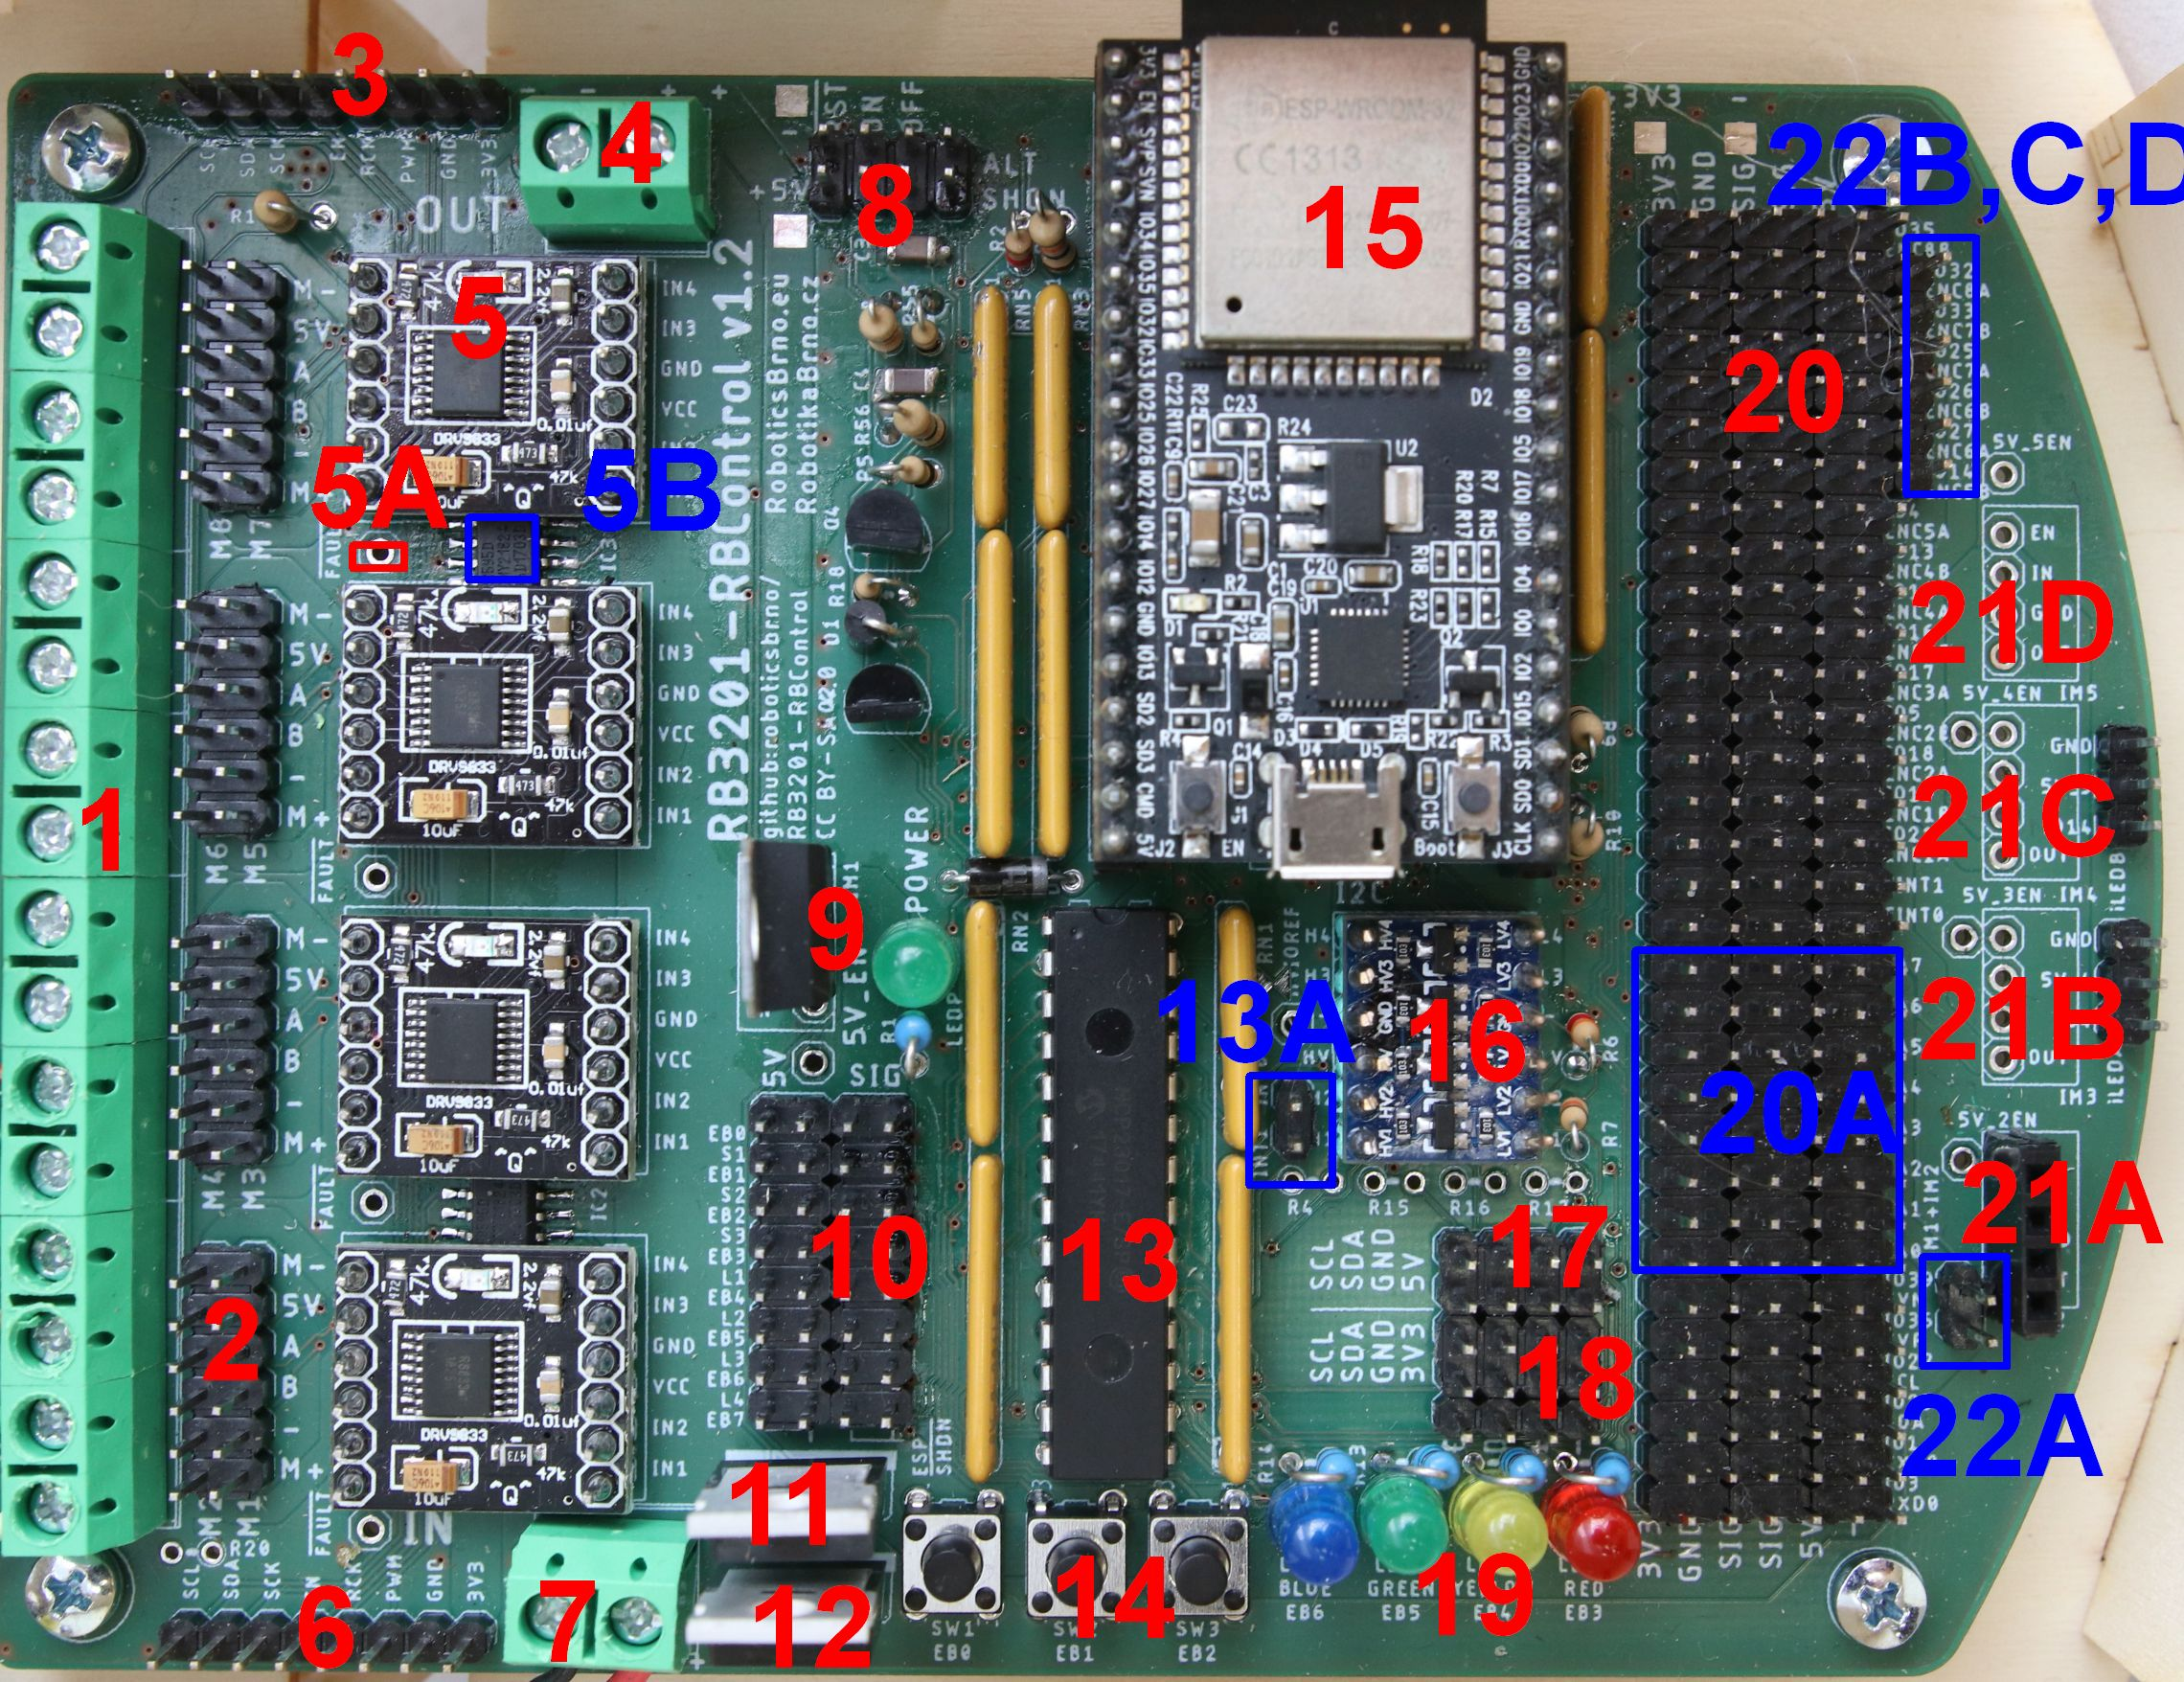
\includegraphics[width=\textwidth]{soubory/RBC_image_description.png}  %todo zmenšit velikost 
 	\caption{Rozložení pinů na desce RB3201-RBControl} 
 	\label{fig:rbc}
 	\end{figure}	


1. Svorkovnice pro připojení DC motorů 

2.  Piny pro připojení motorů s enkodéry. 
Protože ESP32 má málo pinů, je potřeba si zjistit, které piny jsou použité pro enkodéry a nepoužívat je na něco jiného. 

3. Výstupní piny, slouží signálovému propojení s další deskou RBC. 

4. Výstupní napájení. Použije se v případě připojení další RBC desky jako vstupní napájení pro připojenou desku. 
Piny SCL, SDA, GND, 3V3 lze použít i samostatně jako další I2C port.

5. \hyperref[driver]{Drivery} pro DC motory. Každý driver poskytuje PWM napájení pro dva motory. 
Každý driver má vyvedený pin 5A (FAULT), kde je možné měřit, jestli se nenachází v chybovém stavu. 
Každý driver má ochranu proti přetížení i přehřátí $\rightarrow$ při překročení mezních hodnot se vypne. 
Pod drivery jsou posuvné registry 5B, které generují signál pro motory podle pokynů z ESP32.

6. Vstupní piny, slouží signálovému propojení s řídící deskou RBC. 
Piny SCL, SDA, GND, 3V3 lze použít i samostatně jako další I2C port.

7. Vstupní napájení z baterie nebo z řídící RBC desky. 

8. Jde o čtveřici jumperů\footnote{jumper -- propojka mezi dvěma piny \index{jumper} \label{jumper} }, zleva doprava při propojení provedou následující: Reset RBC, zapnutí RBC, vypnutí RBC, vypnutí RBC v případě, že expandér není osazen nebo nefunguje.  

9.  \hyperref[stabilizator]{Stabilizátor} 7805 (dodává cca 1~A, většinu z tohoto proudu spotřebuje RBC pro svůj provoz). Místo 7805 je možné osadit spínaný zdroj, který dodává cca 2~A.

10. Port B z expandéru. 
Zleva doprava jsou to piny: 5~V, GND, 2x signálový pin (ten stejný) na 3,3~V.
Na tomto portu jsou také připojená tlačítka, všechny LED a \textbf{vypínání desky (pin B7)}. Pozor, ve verzi 1.2 jsou popisy pinů posunuté o jeden pin dolů.

11. \hyperref[tranzistor]{Tranzistor} Q1 -- zapíná desku. 

12.  Tranzistor Q3. Po osazení tranzistorem Q3 je deska chráněná proti přepólování.

13. Expandér pinů.
13A jsou piny pro sledování  \hyperref[preruseni]{přerušení}  na portu A a portu B expandéru. 

14. Tlačítka S1, S2, S3. 

15. ESP32-DevKitC

16. Deska, která převádí signál I2C z 3,3~V na 5~V a signál pro připojení inteligentních LED a podobně -- viz č. 17 a 23.

17. 2x I2C na 5~V

18. 3x I2C na 3,3~V

19. 4x LED 

20. Piny pro připojení periferií k ESP32. 
Součástí jsou piny portu A z expandéru (č. 20A). 
Zleva doprava: 3,3~V, GND, 2x signálový pin, 5~V, GND. 
Přitom piny 5~V jsou ve výchozím nastavení připojeny na spínané zdroje (č.21A-D, které samozřejmě musí být osazeny). 

Vyjímka je spodních 8 pinů,
které jsou připojeny přímo ke stabilizátoru nebo spínanému zdroji č. 9. To
také znamená, že na pinech značených 5 V není 5 V, ale tolik voltů, jak
je nastavený stabilizátor, který je připojený k daným pinům. Toto se musí
ohlídat speciálně při připojování serv, jinak je můžete snadno spálit.

Piny IOxx na desce odpovídají pinům na ESP32, piny EXx jsou piny z expandéru pinů, 
EAx jsou volné piny, EBx jsou použité pro tlačítka a diody
(viz popisy na desce a bod č.10) – je potřeba při jejich použití na to dát
pozor.

Popis pinů: například vpravo nahoře: vždy dva popisky odpovídají jedné
řadě, takže například první řada od shora patří k pinu IO35 a současně je na
stejný pin přiveden ENC8B – enkodér pro 8. motor (každý enkodér má dva
výstupy, A a B).

Horní dvě řady pinů jsou připojeny na spínaný zdroj 21D (první řada od
shora je pouze vstupní), dvě řady pinů pod nimi jsou připojeny na 21C,
další dvě řady na 21B a zbývající řady kromě spodních osmi na 21A. Pokud
chceme tyto piny připojit na zdroj č. 9, musíme propojit jumpery 22A-D.
Přitom piny tvoří kaskádu, tj. musím nedřív propojit jumper 22A, potom
22B atd.

21. Místo pro osazení spínaných zdrojů (step-down): 21A, 21B, 21C, 21D.
Každý zdroj má vyvedený tzv. enable-pin. Zdroje jsou ve výchozím stavu
zapnuté a lze je vypnout tak, že na enable-pin přivedu kabelem z jiného pinu
potřebný signál.

Na každý spínaný zdroj (step-expanderdown) je možné připojit jedno servo
nebo dvě mikroserva. Piny jsou vyvedeny tak, aby bylo možné serva připojit
přímo. Přitom zdroj 21D obsluhuje horní dva piny 5 V, zdroj 21C dva piny
5 V pod nimi, zdroj 21B opět dva piny 5 V pod nimi a zdroj 21A všechny
zbývající piny 5 V kromě spodních osmi.

22. Jumpry pro připojení spínaných zdrojů z bodu 21, písmeno vždy odpovídá: 22A, 22B, 22C, 22D.

23. Signál pro inteligentní LED nebo podobné zařízení -- piny na desce nejvíce vpravo (nejsou vyznačeny).

\subsection{Programování a nápověda}
Programování desky RBC –-
viz \url{https://www.mickoflus.cz/guide.html}, sekce programování. Stáhnout,
otevřít a přeložit (build) demo projekt z míčkoflusu, ten si stáhne z GitHubu
všechny potřebné knihovny a bude připraven k překladu.
Příklady kódu: \url{https://rbcontrol.robotikabrno.cz}.

Dokumentace RBControl knihovny: \url{https://github.com/RoboticsBrno/RB3201-RBControl-library}.

\section{Řešení některých problémů}

\subsection{Chyba při uploadu programu do desky Arduino nano:}
 
 Chyba: \\
 {\tt  Please specify 'upload\_port' environment or use global '--upload-port' option}
 
 Řešení: pomohlo spustit příkaz {\tt sudo service udev restart} a znovu spustit VS code a odpojit a připojit desku.  


\begin{thebibliography}{9} \label{literatura}
	
	\bibitem{hr} MALÝ, Martin. \textit{Hradla, volty, jednočipy: úvod do bastlení}. Praha: CZ.NIC, z.s.p.o., 2017. CZ.NIC. ISBN 978-80-88168-23-2. \\
	\url{https://knihy.nic.cz/files/edice/hradla_volty_jednocipy.pdf}

	
	\bibitem{ard} VODA, Zbyšek. \textit{Průvodce světem Arduina}. Vydání druhé. Bučovice: Martin Stříž, 2017. ISBN 978-80-87106-93-8. \\
	\url{https://www.robotikabrno.cz/docs/arduino/Průvodce-světem-Arduina-CZ.pdf}

	\bibitem{citace} \textit{www.citace.com}  [online]
	
\end{thebibliography} % \cite[strana~49]{ard}



